\documentclass[12pt,a4paper]{article}
\usepackage[margin=1.25in]{geometry}
\usepackage{fancyhdr} % fancy header
\pagestyle{fancy} % so fancy
\usepackage[russian,english]{babel} % for russian letters
\usepackage{tipa} % for IPA symbols
\usepackage[round]{natbib} % bibliography
\usepackage{graphicx} % for importing graphics / figures
\usepackage{booktabs} % publication-worthy tables
\usepackage{adjustbox} % makes tables fit nicely on the page
\usepackage{hyperref}
\usepackage{wrapfig}

\lhead{Joshua MEYER}
\rhead{Google AI Follow-up Questions}
\cfoot{} %% make empty to get rid of the page number %% \cfoot{Page \thepage}
\renewcommand{\footrulewidth}{0.4pt} %% this puts a fancy line at the footer


\begin{document}








\subsubsection*{My Research Passion}

\begin{center}
\textit{Everyone should have access to speech technology in their native language.}
\end{center}

This is the conviction that drives my research. I want the world to be a place where someone who's born blind doesn't have to settle for a lesser education because of lack of audiobooks. I've worked with people in that exact situation to build a Kyrgyz speech synthesizer, because this problem is real. I've played a small role to make speech synthesis available for free, but there is a hard limit as to what I can accomplish on my own.

The Google AI residency is the next step towards my goals. I want to publish influential work and get more people caring about low-resource languages. With my knowledge of linguistics and passion for machine learning, the Google Brain team is the perfect place for me to flourish and share my research with others.

Collaborating with researchers at Google, I will help create new approaches and algorithms, testing theories, and diving deeper into multi-task learning. In particular, I have many ideas for multilingual experiments, extracting information from large datasets to transfer knowledge to smaller domains. The competitive (yet collaborative) research atmosphere at Google excites me, and I will bring my enthusiasm and dedication with me. 


\subsubsection*{Open-endness}

My thesis topic is Low-Resource Multi-Task Learning for Deep Neural Network Acoustic Modeling in Automatic Speech Recognition (ASR).

Acoustic models in ASR are classifiers which accept some speech signal (ie. time chunks of an audio file) and return probabilities over phonetic transcriptions. I use a Mutli-Task feedforward neural network (ie. multiple output layers) to perform this classification. Learning related tasks in parallel can improve performance on the main task, because the weights in the net will be biased towards general, task-independent representations of the data (Caruana 1997).

The Multi-Task approach offers an elegant way to exploit small datasets, if you can come up with the right tasks. In my early experiments, I created auxiliary tasks using linguistic theory, lowering Word Error Rates for small data sets. Where previous Multi-Task work found no improvement using linguistic categories, by reformulating the problem I improved over my single-task baseline model ().

The labels in Acoustic Modeling are isolated speech sounds such as \texttt{[b]} or \texttt{[f]}. However, a speech sound is a composite object defined along linguistic dimensions such as vocal chord vibration, tongue placement, lip rounding, turbulence of airflow, etc. Past research created auxiliary tasks by predicting these linguistic dimensions in isolation. This is like taking a 3-dimensional label \texttt{[x,y,z]}, and predicting \texttt{[x]} and \texttt{[y]} and \texttt{[z]} as additional tasks. The problem with this approach is that for the speech signal, the predictive power of any one dimension is very weak.

Reformulating the problem, I created tasks by \textit{removing} one dimension for each task, projecting into \texttt{N-1}-dimensional spaces. That is, instead of \texttt{[x,y,z]} $\rightarrow$ \texttt{[x]} and \texttt{[y]} and \texttt{[z]}, I projected \texttt{[x,y,z]} $\rightarrow$ \texttt{[x,y]} and \texttt{[y,z]} and \texttt{[x,z]}. This approach improves performance, lowering Word Error Rates. These \texttt{N-1}-dimensional spaces have more predictive power, and force the net to learn the paticularities of each dimension.

However, defining each task by hand is not a scalable approach. Since then, I've devoted my research to finding scalable, automatic solutions to task creation.

\subsubsection*{Mutli-Task as Ensemble}

A Multi-Task classifier is a special case of an ensemble model, where the feature extractors are trained in parallel. Once I made that connection, I found a mass of inspiration from past ensemble work. Looking for \textit{scalable} ensemble model approaches, I came across the Random Forest.

A Random Forest is created by training multiple trees on random re-samples of the data. Each subsample has its own decision plane, specific to its particular data and noise. By voting among all trees, noise is ignored but data generalities remain. Extending this approach, my current research investigates Multi-Task neural nets, where the tasks are random subsets of the data.


\begin{wrapfigure}{L}{0.375\textwidth}
\centering
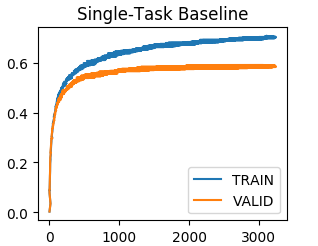
\includegraphics[width=0.35\textwidth]{figs/stl.png}
\end{wrapfigure}

 I use the Kaldi Speech Recognition toolkit to run experiments. The figure to the left is my current baseline model performance with a 5-layer Time-Delay Neural Network, with 200 dimensional hidden layers. The x-axis is number of iterations, and the y-axis is audio-frame classification accuracy. This model has overfit the training data. We can see the accuracy on training data increases, while accuracy on held-out validation data is stagnant and eventually decreases. 


\begin{wrapfigure}{R}{0.4\textwidth}
  \centering
  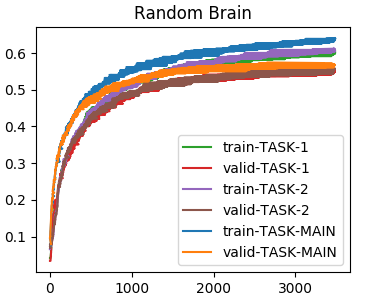
\includegraphics[width=0.35\textwidth]{figs/mtl.png}
\end{wrapfigure}

To the right is the performance of my Multi-Task model (which I have dubbed the Random Brain). This model is currently training on an Amazon instance with 30 auxiliary tasks (I am only showing 2 auxiliary tasks here). The tasks are random, 50\% subsets of the dataset (5 hours of speech). The main task is the entire dataset. My impressions from this early data are the following: classification accuracy is lower for MTL than the Single-Task model, but after 3,500 iterations we see less plateauing than in the baseline. This could mean the extra tasks are a hinderance making the task harder to learn, or they are penalizing overfitting, and given enough iterations the Multi-Task model will beat out the baseline. If this approach works, then the Random Brain could be used to train \textit{any neural net} on \textit{any dataset}. I 'm cautiously optimistic, because I want to find solutions which can impact the field as a whole, not just speech recognition.


The open-endedness of research does not phase me. I know my goal (make speech technology for all languages), and I know it is so big that I can happily spend a career chipping away at it, and Google AI is the perfect place to start chipping. 



\begin{center}
\textit{Thank you for your time and consideration.}  
\end{center}
\end{document}



 
